
%
%  $Description: Author guidelines and sample document in LaTeX 2.09$ 
%
%  $Author: ienne $
%  $Date: 1995/09/15 15:20:59 $
%  $Revision: 1.4 $
%

\documentclass[times, 10pt,twocolumn]{article} 
\usepackage{latex8}
\usepackage{times}

\usepackage{amsfonts}
\usepackage{amsmath}
\usepackage{boxedminipage}
%\usepackage{epsf}
\usepackage[latin1]{inputenc}
%\usepackage{babel}
\usepackage{graphicx}
\usepackage{setspace}
\usepackage{hyphenat}


%\documentstyle[times,art10,twocolumn,latex8]{article}

%------------------------------------------------------------------------- 
% take the % away on next line to produce the final camera-ready version 
\pagestyle{empty}

%------------------------------------------------------------------------- 
\begin{document}

\title{Analysis of Cache Compression on Embedded Applications}

%\author{Anderson Briglia\\
%Universidade Federal do Amazonas\\ Departamento de Ci�ncia da Computa��o \\ Av. 
%General Rodrigo Otavio, Manaus-Amazonas, Brazil\\ anderson.briglia@gmail.com\\
% For a paper whose authors are all at the same institution, 
% omit the following lines up until the closing ``}''.
% Additional authors and addresses can be added with ``\and'', 
% just like the second author.
%\and
%Edward David Moreno\\
%DCOMP - Departamento de Ci�ncia da Computa��o\\
%Universidade Federal de Sergipe\\ edwdavid@gmail.com\\
%}

\maketitle
\thispagestyle{empty}

\begin{abstract}
\nohyphens{
Memory compression has been used since applications memory demand increases over the time. Embedded systems has limited resources, processing and memory capacity are example of this. With hardware minituarization and embedded systems improvements, it is easy to have multimedia applications running in embedded computers like PDA's or Internet tablets. The work evaluated in this paper is called Compressed Cache and it acts in RAM memory of mobile devices running Linux as Operating System. Compressed Cache has been used to virtually increase the amount of RAM memory available to user applications, avoiding critical memory situations and providing more scenarios for multimedia applications. This paper shows an evaluation of Compressed Cache regarding performance, memory behaviour and improvements brought by RAM memory compression. MiBench benchmarks are also used to evaluate the Compressed Cache memory operations.
}
\end{abstract}


%------------------------------------------------------------------------- 
\section{Introduction}
\nohyphens{
Most of embedded systems has as common characteristic: your usage for single specific tasks. But embedded systems for general purpose are pretty common as well \cite{mor00}. In the past, embedded systems were used to perform single tasks, for example: DVD players firmware, camera systems, cars control, etc. But over the years this kind of equipment becomes more and more powerful in terms of processing and data storage. Due this, we have PDA's (Personal Data Assistant), internet tablets and netbooks which have the same processing capacity of old desktop computers. Users applications used on embedded systems have your requirements increased as well. Multimedia and Internet access is almost mandatory for embedded systems and user applications. Given this scenario, it is important to study ways to improve the user experience when using an embedded system. This paper evaluates one of the purposes for embedded systems which have to provide high processing power and memory capacity for user applications.
%}
%\nohyphens{

Linux is an Operating System developed by a young student, Linus Torvalds, in University of Finland - Helsink \cite{linux:09}. Linus used Minix (another operating system), as basis and implemented Linux with new features. Linux kernel is released under GPL (GNU Public License), and the source code is available for everyone. As developers have access to Linux kernel, this operating system supports a largely number of hardware architectures, since single-processor machines to multi-processor ones. Due this, Linux has been used in embedded systems like PDA's, internet tablets, netbooks, etc.
%}
%\nohyphens{

Compressed Cache (Compcache) adds a new level on Linux memory hierarchy \cite{castro03, douglis93, kaplan99compressed}. Compcache is used to improve the access time to memory pages in Linux kernel when storing such pages in RAM (Random Access Memory} and/or to improve the memory storage capacity, compressing pages in a virtual memory area called ramzswap. Swap areas are generally used as RAM extensions using block devices (hard disks, flash memory, etc), to store memory pages. But swap areas has a cost: pages input/output (I/O) velocity rates. It is knowing that block devices are slower for I/O operations due to technology used to store data. RAM memory is faster than block devices and keeping more memory pages in RAM brings more velocity when some page is requested by some application.
%}
%\nohyphens{

The evaluated project presented in this paper uses a virtual swap area allocated in RAM to store memory pages in a compressed format. The tests presented here intend to show that, even with compression/decompression overhead added by Compcache, the page access time is smaller than have the same page stored in a block device. It is evaluated as well the behavior of Compcache when memory is consumed.
%}
%\nohyphens{

As presented in \cite{briglia07}, not only input and output rates could be improved when Compcache is used, but also the system behavior. Especially in memory-critical cases leading, Compcache can be used to ameliorate the Out-of-memory conditions. The Compcache version evaluated in \cite{briglia07} was updated and this new version is evaluated in this paper. Since Compcache had important modifications, it is important to evaluate it again and analyze if this new version had some improvement. The major difference between Compcache version used in \cite{briglia07} and the version evaluated here, is the implementation of a virtual swap area called ramzswap. Using this new approach, it is not necessary to make modifications in the Linux kernel, and ramzswap takes advantage of existent swap system. Another contribution by this paper are the tests performed using MiBench \cite{GRE01} to evaluate the memory consumption behavior. Since MiBench is largely used in embedded systems evaluations, this paper presents Compcache usage against MiBench benchmarks and tests using new Compcache version. Experiments used in this work are based in Briglia's\cite{briglia07} tests.
%}
%\nohyphens{

This paper has been organized in six sections: Introduction, Linux Virtual Memory Overview, Compressed Cache Implementation Design, Experiments, Related Wor and Conclusion. The second section presents how Linux virtual memory system is implemented and used by Compcache. The second section shows how Compcache is designed to use virtual memory system as compressed area for memory pages. The third section presents all experiments done in this paper: memory consumption tests, MiBench tests, etc. Related Word section presents some information about previous compressed cache implementations. And the last section evaluates how Compcache acted upon critical memory leads.
}
%------------------------------------------------------------------------- 
\section{Linux Virtual Memory Overview}
\nohyphens{
Physical pages are the basic unit of memory management \cite{love05kerneldevel} and the MMU (Memory Management Unit) is the hardware that translates virtual pages addresses into physical pages address and vice-versa. This compressed caching implementation, Compcache \cite{ccache09}, takes advantage of swap system to store compressed pages into a virtual swap partition. When the system is under a low memory condition, it evicts pages from memory. It uses Least Recently Used (LRU) criteria to determine order in which to evict pages. It maintains two LRU lists---active and inactive LRU lists. These lists may contain both page-cache (file-backed) and swap-cache (anonymous) pages. When under memory pressure, pages in inactive list are freed as:

\begin{itemize}
\item Swap-cache pages are written out to swap disks using swapper\_space writepage() (swap\_writepage()).

\item Dirty page-cache pages are flushed to filesystem disks using filesystem specific writepage().

\item Clean page-cache pages are simply freed.
\end{itemize}
}
%\subsection{About Swap Cache}

%\nohyphens{
%This is the cache for anonymous pages. All swap cache pages are part of a single swapper\_space. A single radix tree maintains all pages in the swap cache. swp\_entry\_t is used as a key to locate the corresponding pages in memory. This value identifies the location in swap device reserved for this page.
%}

%\subsection{About Page Cache}
%\nohyphens{
%This is the cache for file-system pages. Like swap cache, this also uses radix-tree to keep track of file pages. Here, the offset in file is used as the search key. Each open file has a separate radix-tree. For pages present in memory, the corresponding radix-node points to struct page for the memory page containing file data at that offset.
%}

\subsection{Compressed Cache Overview}
\nohyphens{
Compressed Cache (Compcache), is a technique which adds a new level in Linux memory hierarchy \cite{castro03, douglis93, kaplan99compressed}. Compcache is used to improve the memory pages access time in Linux kernel, storing more pages in RAM memory instead of slow block devices (used in regular swap\footnote{Swap area is a reserved portion from the filesystem which intends to increase the available virtual memory amount, improving the free memory for user applications.} areas) and avoiding that more pages were discarded. It is known that swap areas are slower than main memory, because block devices (usually hard disks), have higher access time rates for Input/Output operations. For embedded systems the problem is worst since swap area is generally not present in such systems.
%}
%\nohyphens{

Using the same compression algorithm present in JFFS2 filesystems (LZO \cite{obe05lzo, ZivLem77}), swap selected memory pages are compressed and sent to the virtual swap area, called ramzswap. This virtual swap acts like a block device with a swap partition and from Linux kernel point of view, there is no difference from a regular swap partition and ramzswap swap partition. Virtual compressed swap is self-contained and the compression and decompression is done when a page is inserted or retrieved from Compcache. See Figure \ref{fig:compcache}.
}

\begin{figure}[htb]
 \centering
 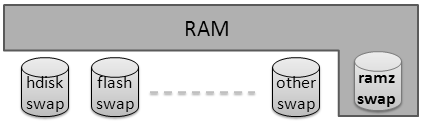
\includegraphics[scale=0.5]{figs/sbac-compcache.png}
 % compcache.png: 425x122 pixel, 72dpi, 14.99x4.30 cm, bb=0 0 425 122
 \caption{Swap with virtual block device -- ramzswap \cite{ccache09}.}
 \label{fig:compcache}
\end{figure}

\section{Compressed Cache Implementation Design}

\nohyphens{
A virtual block device is configured to have a swap partition and is added to system swaps table. Doing this, the PFRA is used to select the swappable pages and sent them to virtual compressed area (ramzswap).

To avoid fragmentation and improve efficiency, a new memory allocator was developed for Compcache. xvMalloc \cite{ccache09} is based on TLSF (Two Level Segregate Fit) allocator \cite{Masmano04}, which was developed for real-time systems.

General purpose memory allocator, generally are designed to handle allocations bigger than 4 kilobytes, which is the default size for memory pages, on Linux. This new allocator, xvMalloc, is designed to work with very tiny memory allocations, for example 32 bytes, or $3/4$ of default page size. Due to this page size characterist, fragmentation must be avoided since performance is an important issue.

Inherited from TLSF \cite{Masmano04}, xvMalloc \cite{ccache09} has some useful features that are used in Compcache:

\begin{itemize}
\item O(1) Alloc/Free: Except for cases where xvMalloc has to go to system page allocator to get additional memory.
\item Very low fragmentation: In all tests, xvMalloc memory usage is within 12$\%$ of ``Ideal'' allocator.
\end{itemize}
}

\nohyphens{
But, xvMalloc has added new features \cite{ccache09}, as follow:

\begin{itemize}
 \item Allocation size is always in range [MIN, MAX] and this is range is small. For Compcache this range is, for example $[32, 3/4 * PAGE\_SIZE]$. This avoid fragmentation.
 \item Memory being managed is not backed by any VA. Allocator records $<$pageNum, offset$>$ for each object.
 \item Per object overhead is 4 bytes. In TLSF, this value is 16 bytes.
 \item xvMalloc stores \textbf{exact} object size in object header. This saves additional 2 bytes per object since it is not necessary to store data section beginning.
\end{itemize}

From kernel point-of-view, ramzswap is a normal swap area and must provide a small access time for compressed pages. Low fragmentation results in less time when a compressed page is required by the memory management system. Another important feature implemented by xvMalloc is the size of meta-data for each object. With 4 bytes for each object (or compressed page), more space can be used to store compressed pages itself. The Compcache version presented in \cite{briglia07}, meta-data size is an issue because important bytes were spent to address the compressed pages.
}

%------------------------------------------------------------------------- 
\subsection{Compressed Pages Storage}
\nohyphens{
Compressed pages are stored in data structures which xvMalloc handles. These structures are designed to group similar pages: free pages and compressed pages.
Object header used by xvMalloc to handle compressed pages is showed in Figure \ref{fig:obj-header}.

\begin{figure}[htb]
	\centering
	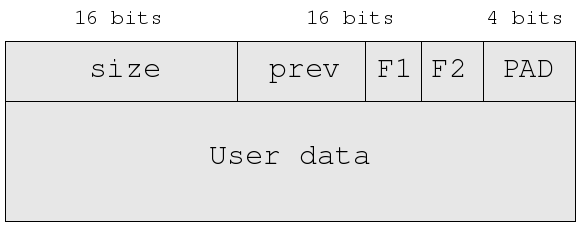
\includegraphics[scale=0.5]{figs/sbac-obj-header.png}
	\caption{Object header handled by Compressed Cache memory allocator-- xvMalloc.}
	\label{fig:obj-header}
\end{figure}

Where, each field means \cite{ccache09}:

\begin{itemize}
 \item Size: compressed page size calculated by compressor and used by xvMalloc.
 \item Prev: offset of previous used/free block (relative to beginning of page).
 \item \textit{Flags}:
	\begin{itemize}
		\item F1: flag used to indicate if a block is being used or not.
		\item F2: flag used to indicate if the previous block is being used or not.
	\end{itemize}
 \item PAD: Not required if ALIGN if 4 bytes.
\end{itemize}

The total size for data structure used to represent a compressed page is 4 bytes.
Free objects use a different object header. It is represented in Figure \ref{fig:obj-free}.

\begin{figure}[htb]
	\centering
	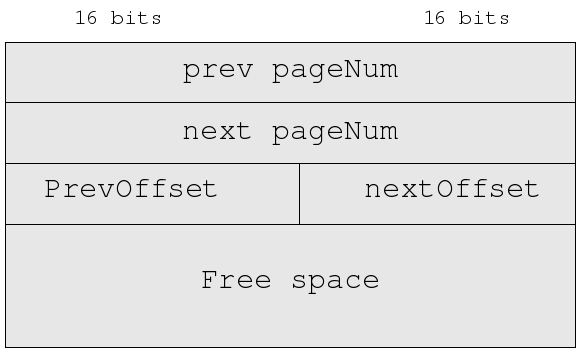
\includegraphics[scale=0.5]{figs/sbac-obj-free.png}
	\caption{Free object header.}
	\label{fig:obj-free}
\end{figure}

Each page represented by Figure \ref{fig:obj-free} is identified by \textit{$<$pageNum, offset$>$} tuple. It is used to quickly find a compressed page inside Compcache memory area.
}

\subsection{Insertion and Removal Pages Operations}
\nohyphens{
\textbf{Compressed pages insertion:} first, selected page is compressed and copied to a buffer page. Compression algorithm used to compress is LZO \cite{obe05lzo, ZivLem77}, which is already implemented by Linux kernel. After the compression, Compcache sends the compressed page to ramzswap virtual swap area. At this moment, ramzswap calls xvMalloc passing compressed page size. xvMalloc allocates a memory portion with exact size of compressed page. Now, the compressed page is represented by the data structures discussed previously in this paper. After all the insertion process finishes, a tuple containing page number and offset is returned by xvMalloc to Linux kernel virtual memory system, which inserts this identifier into the radix-tree used to store swapped memory pages. Figure \ref{fig:radix-tree} shows the VM radix-tree before compressed page identifier is inserted.

\begin{figure}[htb]
	\centering
	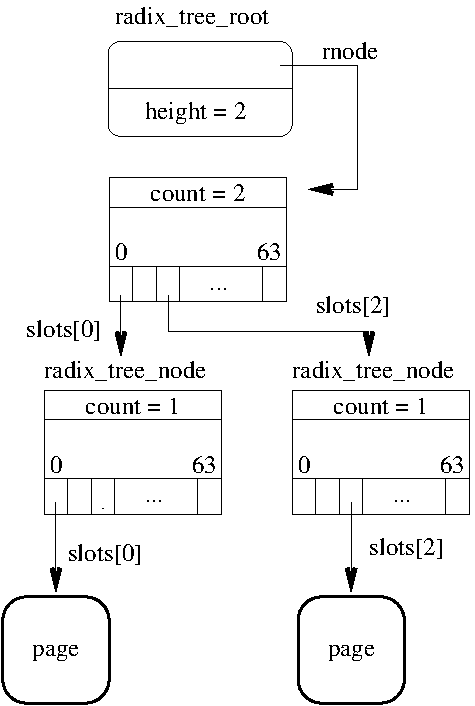
\includegraphics[scale=0.6]{figs/radix_tree}
	\caption{Radix-tree: before compressed page is stored.}
	\label{fig:radix-tree}
\end{figure}

\textbf{Compressed pages removal:} from PFRA and kernel point-of-view, there is no difference between compressed and regular pages represented in radix-tree. Actually, the difference is that compressed pages are swapped to ramzswap virtual swap area. This way, the compressed page reference passed to radix-tree is not different from a regular swapped page. All decompression and compression operations are done in block device level, with no alterations on higher levels, like kernel virtual memory. Another gain using this approach is the fact that Compcache uses actual kernel system to locate all compressed pages when necessary, adding just decompression overhead when page is required.
}
\section{Experiments}
\nohyphens{
This section we will present the tests used to evaluate Compcache running in an embedded Linux system. The main goal for the tests is to evaluate the impacts and memory consumption behavior when system has a compressed memory area available. The experiments are also to evaluate some characteristics, as follow:

\begin{itemize}
	\item How many pages are kept by Compcache and do not go to real swap partition, avoiding slow I/O operations.
	\item In wich situations Compcache could avoid OOM (Out-of-memory killer), to be called.
	\item What is the Compcache compression/decompression overhead.
\end{itemize}

As said before, Compcache implementation handles all swappable pages. Making measurements using swap in/out operations is possible to evaluate Compcache behavior and performance.

To evaluate Compcache, we did a comparison between a real swap against Compcache's virtual swap (ramzswap). To store the swap partion using real swap, MMC cards\footnote{The MMC cards are used as secondary memory for mobile devices, cameras, etc. MMC cards have a read/write rate up to 52 MB/seg. The storage capacity varies from some megabytes to gigabytes.} were used. This comparison was used to measure the overhead added by Compcache when pages are swapped in/out from ramzswap.
}
\subsection{Test suite and Methodology}
\nohyphens{
As test platform, a mobile device were used. It runs embedded Linux as native operating system. Nokia Internet Table N810 \cite{nokiaN810} has an ARM1136 processor, 400Mhz, 128MB RAM memory and 256MB of flash memory, used as secondary storage. This device still have 2D/3D graphics accelerator but it was not evaluated, and has two MMC/SD cards slots.

As we can see on device's specification, it is focused on multimedia usage. As we know, multimedia applications have high processor and memory usage rates. The tests intend to use memory intensively, hence we can measure the Compcache impact on system performance. The tests were divided into two groups: tests with real applications and tests using synthetic benchmarks. Tests with real applications tried to simulate a high memory consumption scenario with a lot of applications being executed and with some I/O operations to measure the memory and power consumption behavior when Compcache is running. Synthetic behchmarks were used to evaluate the Compcache performance, once they provided a easy way to measure the time spent on the tests.

Tests with real applications consist of:

\begin{itemize}

\item Running 8 or 9 Opera browsers and load some pages through a wireless
      Internet connection.
\item Playing a 7.5MB video on Media player.
\item Execute a media player to play mp3 audio, index media files and open pictures.
\item Opening a PDF document.
\end{itemize}

We used an application called \textbf{xautomation} \cite{xauto07} to interact with the X system through bash scripts from the command line. Xautomation controls the interface, allowing mouse movements, mouse right and left clicks, key up and down, etc. Reading the \ident{/proc/meminfo} file, we have the memory consumption, and some graphics related to the memory consumption can be plotted. They will be shown and commented on in the following sections.

The tests using synthetic benchmarks were executed using MemTest~\cite{memtest06}. MemTest is a group of small tests to evaluate the stability and consistency of the Linux memory management system. It contains several tests, but we used just one, since the main goal is to measure the Compcache performance: \textbf{fillmem}. This test intends to test the system memory allocation. It is useful to verify the virtual memory system against the memory allocation operation, pagination, and swap usage. It has one parameter which defines the size of memory allocated by itself.

Still using synthetic benchmarks, MiBench \cite{GRE01} was used. Since MiBench is largely used to evaluate embedded system performance, some measurements executing MiBench utilities were done.

All the tests, using real applications or synthetic benchmarking, were applied using a pre-configured scenarios, depending on what would be measured. Basically there are scenarios with different RAM memory sizes, with or without a \textit{real} swap partition, and with or without Compcache added to the system.

Memory behavior tests evaluate the memory consumption against time and the OOM killer interaction on the scenarios discussed before. Performance tests used MemTest \cite{memtest06} to measure the total time of the \texttt{fillmem} execution.
}
\subsection{Memory Behavior Tests}
\nohyphens{
The main goal of these tests is to see what is happening with the memory when Compcache is compressing and decompressing pages. To execute the tests real application scenarios were used, using applications provided by the default installation of the N810's distribution.

To plot the graphs presented in this section, measurements through \texttt{procfs} reading were done, collecting information about MemFree and memory used by Compcache virtual swap (ramzswap).

Figure \ref{fig:behavior-test} shows the memory consumption againt time with Compcache size configure to 1024 pages or 4MB.

\begin{figure}[htb]
 \centering
 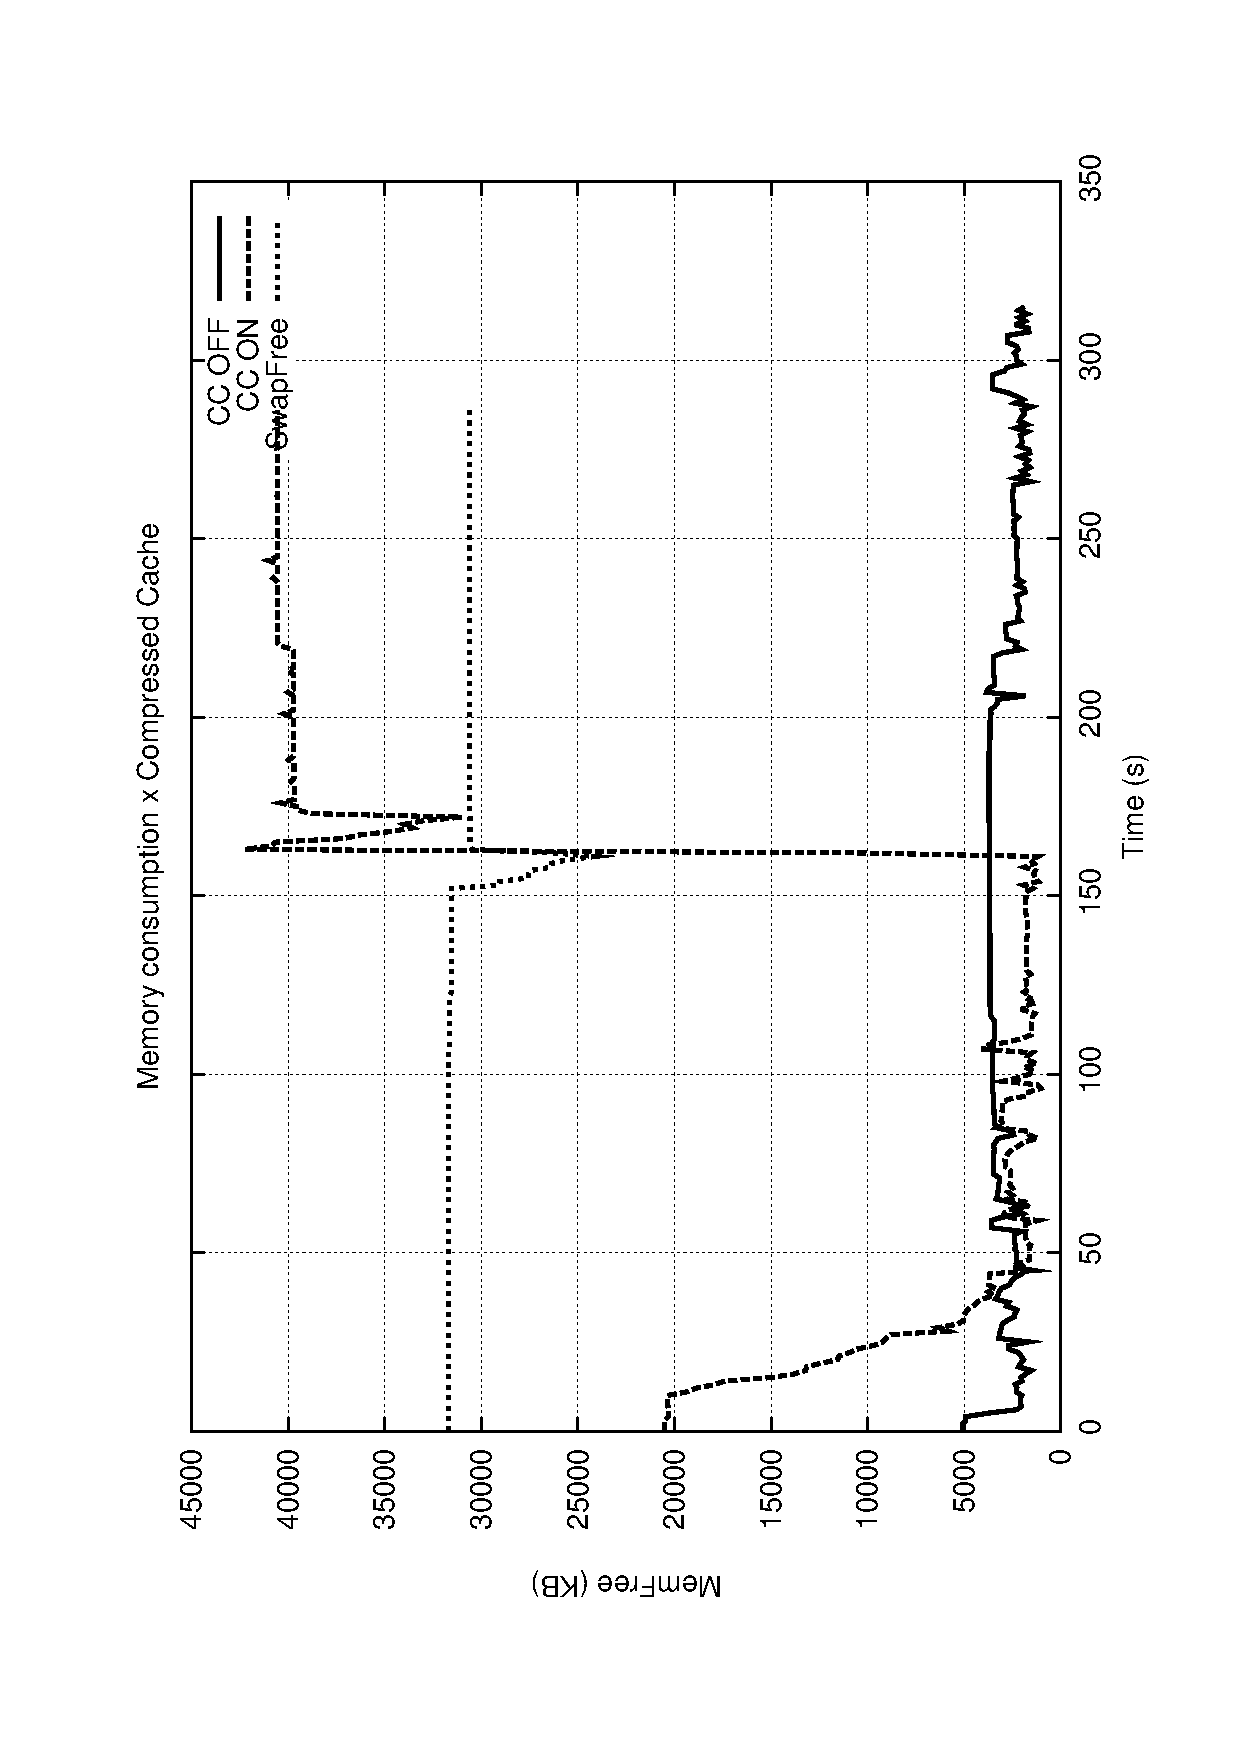
\includegraphics[scale=0.32]{figs/sbac-behavior-no-cc}
 % behavior-no-cc.png: 640x480 pixel, 72dpi, 22.58x16.93 cm, bb=0 0 640 480
 \caption{Memory behavior test using Compcache.}
 \label{fig:behavior-test}
\end{figure}

As can be noticed in Figure \ref{fig:behavior-test}, Compcache has used a portion of free memory to allocate virtual swap space. Due this, free memory available to system is smaller when Compcache is on. On critical memory situations, this smaller free memory can be hazardous since OOM can be called faster to free memory.

After half test duration, as seen in Figure \ref{fig:behavior-test}, there was a faster memory consumption increase, even in virtual swap area. But, Compcache was unable to avoid the OOM call and due this, some memory is freed when free memory targets very low rates.
}

\subsection{Performance Tests}
\nohyphens{
Performance tests aim to analyze the Compcache overhead: compression overhead, ramzswap handling overhead, and page recovery overhead. With these tests it is expected to prove that Compcache, even with all those overheads, is faster than using a swap partition on a block device.

To test memory allocation speed, was used a program from MemTest \cite{memtest06}, called \textbf{fillmem}. Fillmem was used to make memory allocation very fast. In Figure \ref{fig:fillmem50}, fillmem execution time is represented. Memory allocation amount is equal to 50MB.

\begin{figure}[htpb]
 \centering
 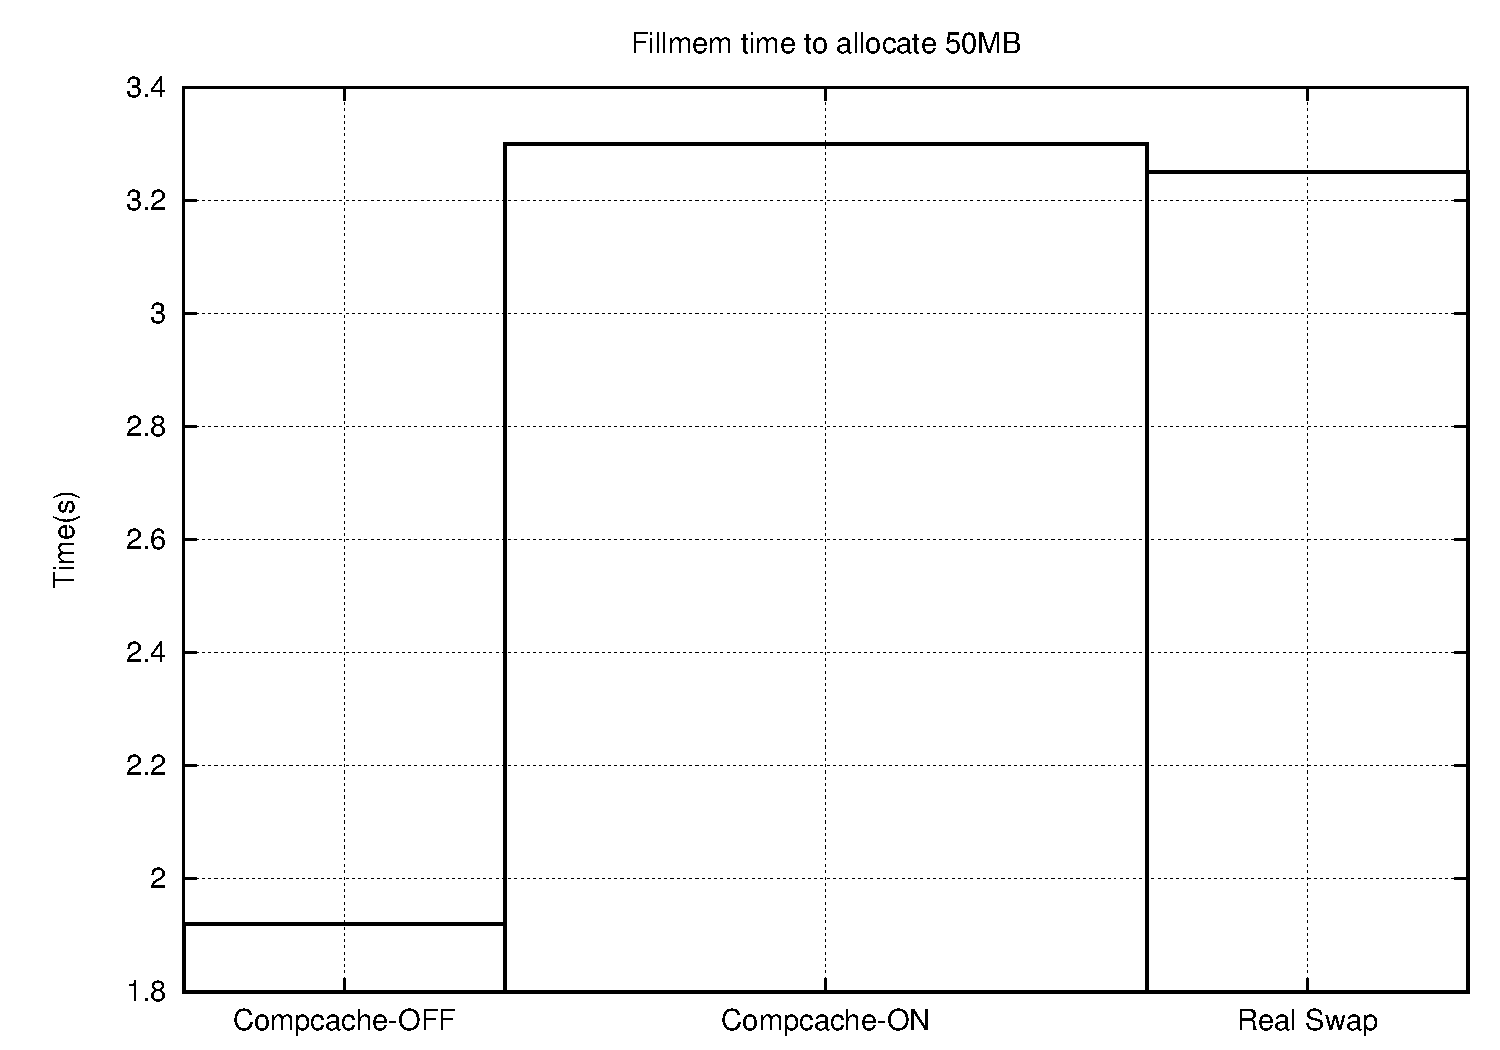
\includegraphics[scale=0.32]{figs/sbac-fillmem50}
 % fillmem50.png: 640x480 pixel, 72dpi, 22.58x16.93 cm, bb=0 0 640 480
 \caption{Fillmem execution time to allocation 50MB.}
 \label{fig:fillmem50}
\end{figure}

At the graph showed in Figure \ref{fig:fillmem50}, can be noticed that execution time for fillmem to allocate 50MB of memory is three times bigger when Compcache is on. It happened since Compcache using ramzswap has some overheads to compress/decompress pages and calculate all page addressing. As seen before, the device used in tests \cite{nokiaN810}, does not have a hard disk for swapping. Due this, flash memory and MMC memory were used as real swap partition. But flash memory and MMC memory have access rates much bigger than hard disk ones. The difference between access a page stored in an MMC card, flash memory or RAM memory is very small. This difference is much bigger when hard disks are used as real swap.

Even the ramzswap pages retrieval had a time slightly bigger than when real swap was used. It happened due to decompression overhead added by Compcache.

\subsection{Using MiBench to test Compressed Cache}
MiBench \cite{GRE01} is a set of synthetic benchmarks which simulates several types of operations. MiBech intends to test hardware architecture performance and embedded systems.

The major difference between MiBench and other embedded system benchmarks, is that the first one is composed with Open Source utilities to make all measurements and tests. Another difference is that MiBench is subdivided into various modules \cite{GRE01} grouped by the test target, see below:

\begin{itemize}
 \item \textit{Automotive and Industrial Control}: groups utilities to test microprocessor dedicated to control embedded systems. This category have programs which test arithmetic operations, bit counting, ordering operations and image processing. 
 \item \textit{Network}: this category has programs to test routers microprocessors, tree search operations and algorithms used in switches.
 \item \textit{Security}: category used to evaluate encrypt algorithms, decrypting, and hash operations of a microprocessor.
 \item \textit{Consumer Devices}: this category has programs which evaluate image processing, HTML rendering and audio playback.
 \item \textit{Office Automation}: groups programs used to test text operations such as used in office equipments, like printers, copiers, etc.
 \item \textit{Telecommunications}: this category contains programs used to test microprocessors used in telecommunication devices. 
\end{itemize}

Tests done in this section intend to evaluate if Compcache has impact on MiBench benchmarking and, see if this impact good or prejudicious. Even the device used in these tests does not fit in all MiBench categories, was decided to test one program from each category. This way, we should have a better panorama of MiBench utilization when Compcache is added to an embedded system.
Next graphs show the Compcache usage versus time when MiBench benchmarks were executed.

\begin{figure}[htpb]
 \centering
 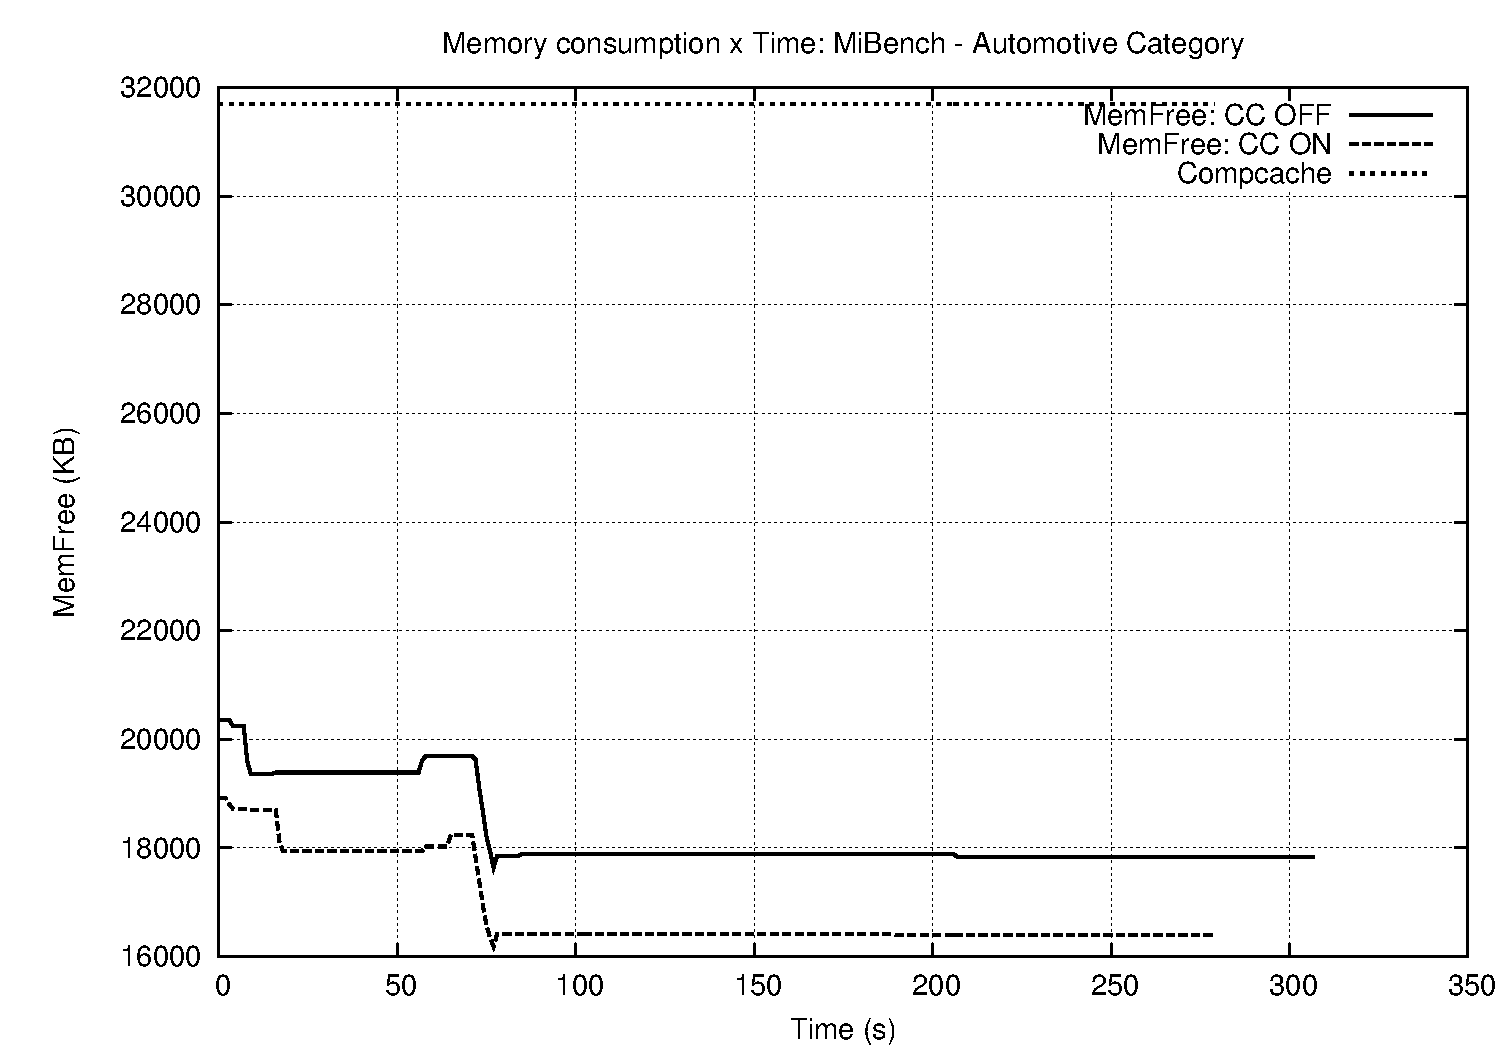
\includegraphics[scale=0.32]{figs/sbac-automotive}
 % automotive.png: 640x480 pixel, 72dpi, 22.58x16.93 cm, bb=0 0 640 480
 \caption{Compcache usage: Automotive benchmarking}
 \label{fig:mibench_automotive}
\end{figure}

\begin{figure}[htpb]
 \centering
 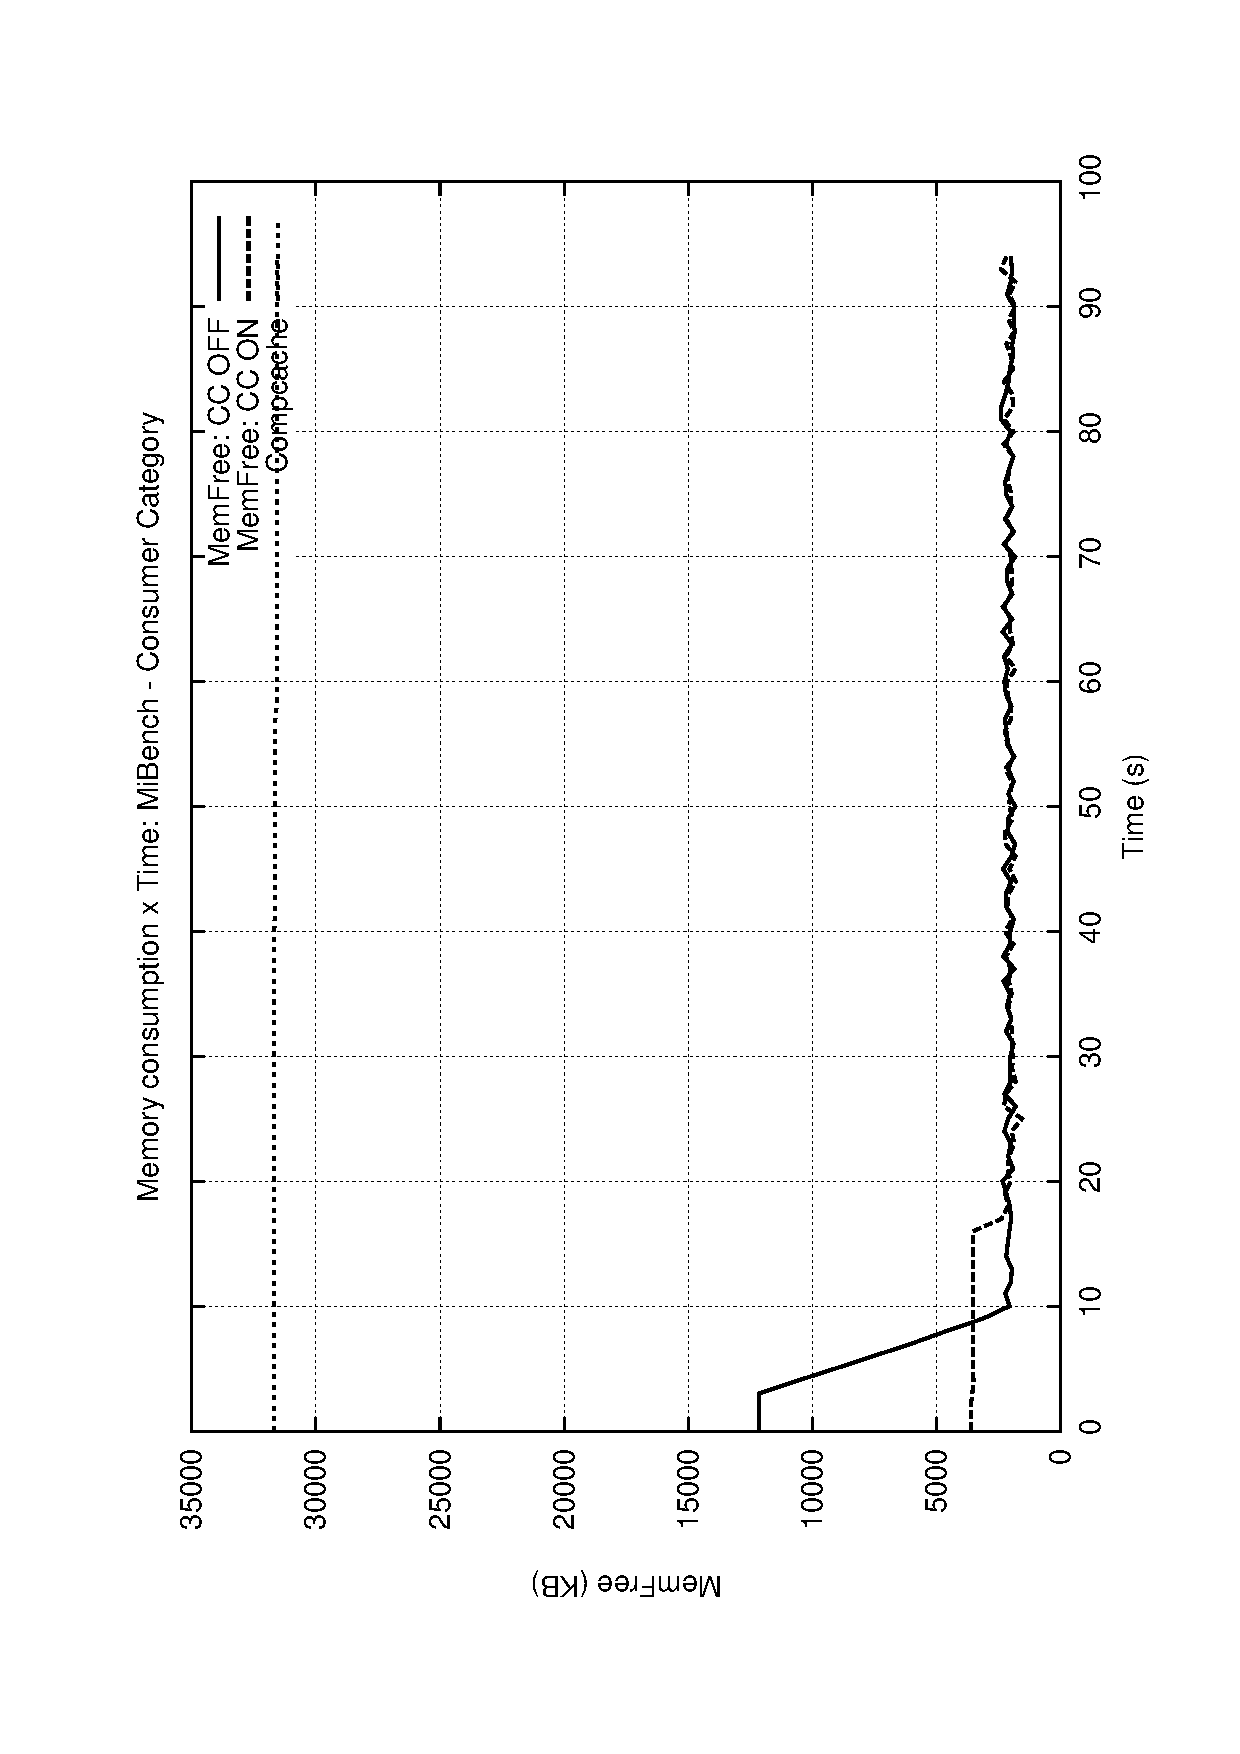
\includegraphics[scale=0.32]{figs/sbac-consumer}
 \caption{Compcache usage: Consumer benchmarking}
 \label{fig:mibench_consumer}
\end{figure}

\begin{figure}[htpb]
 \centering
 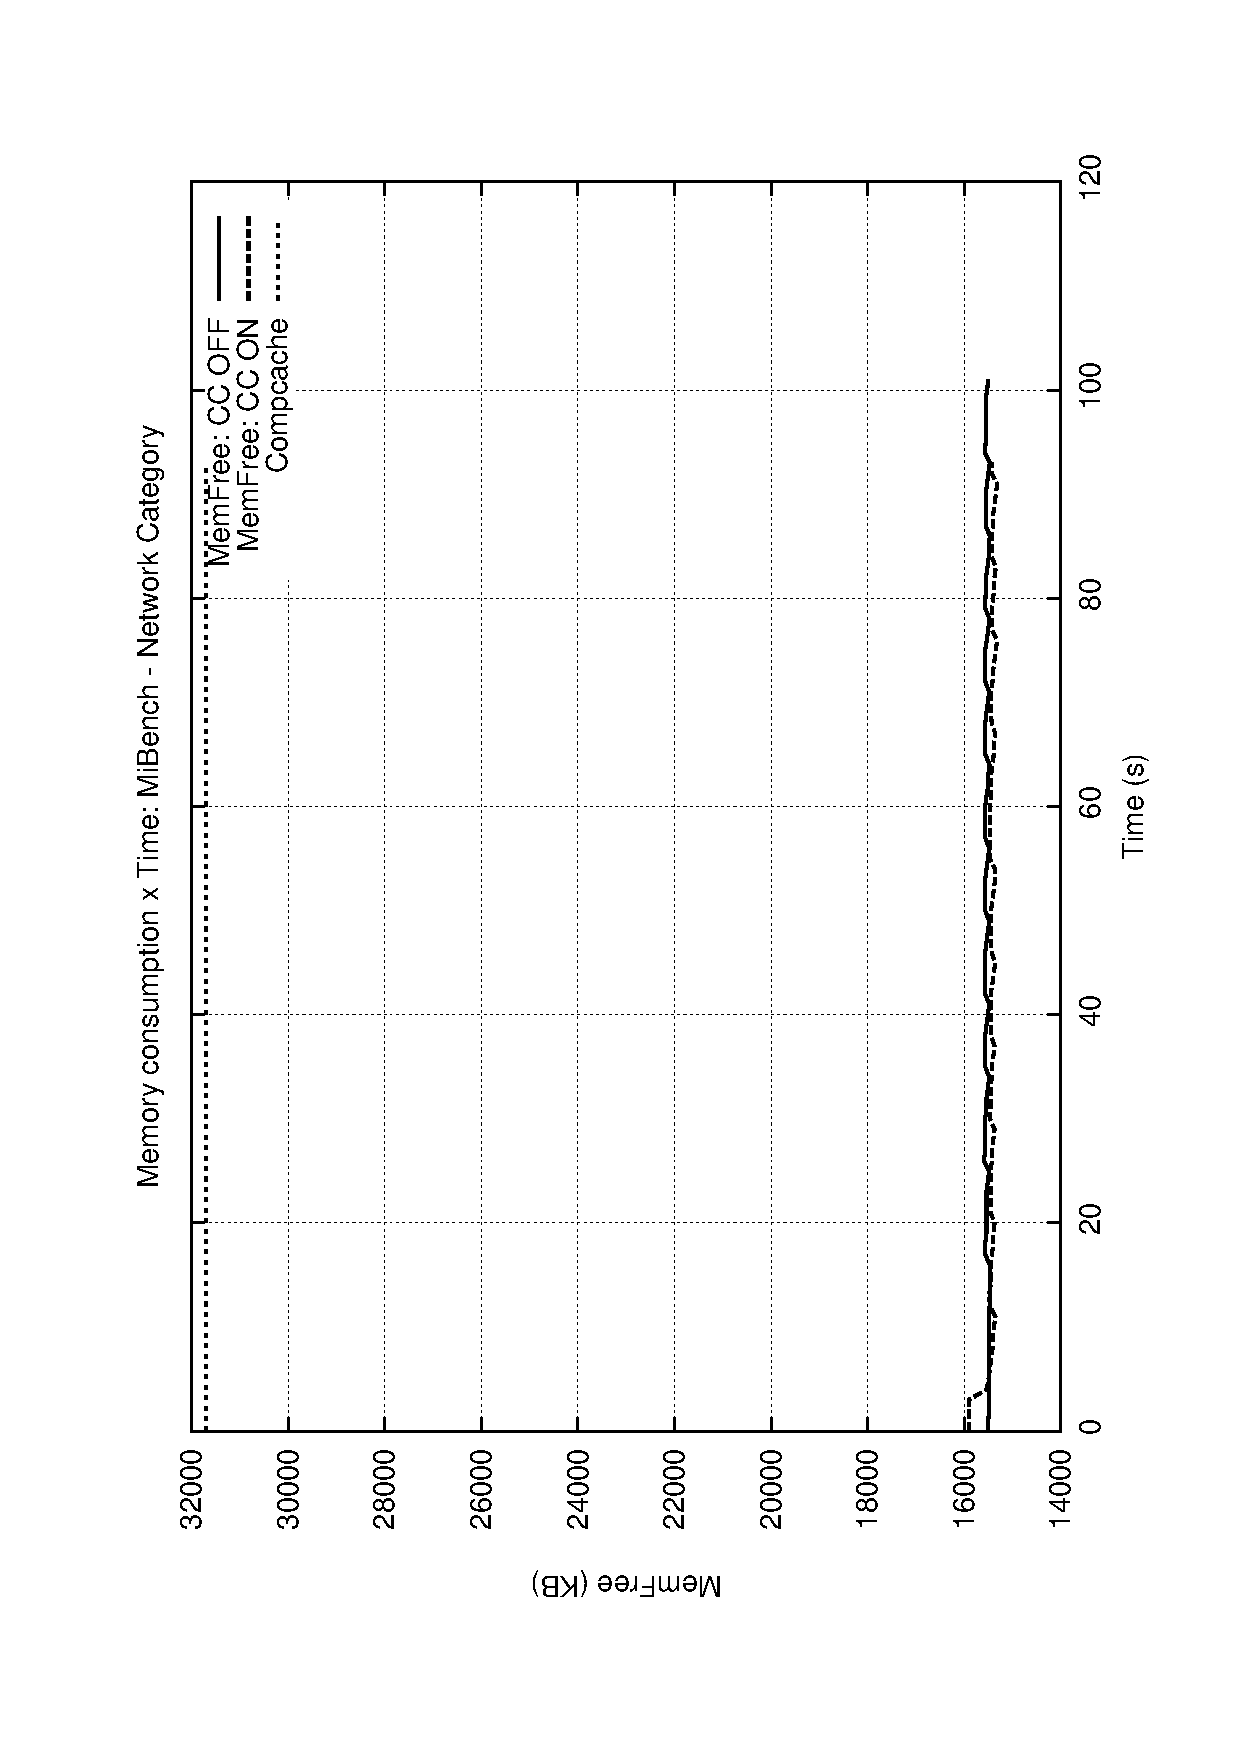
\includegraphics[scale=0.32]{figs/sbac-network}
 \caption{Compcache usage: Network benchmarking}
 \label{fig:mibench_network}
\end{figure}

\begin{figure}[htpb]
 \centering
 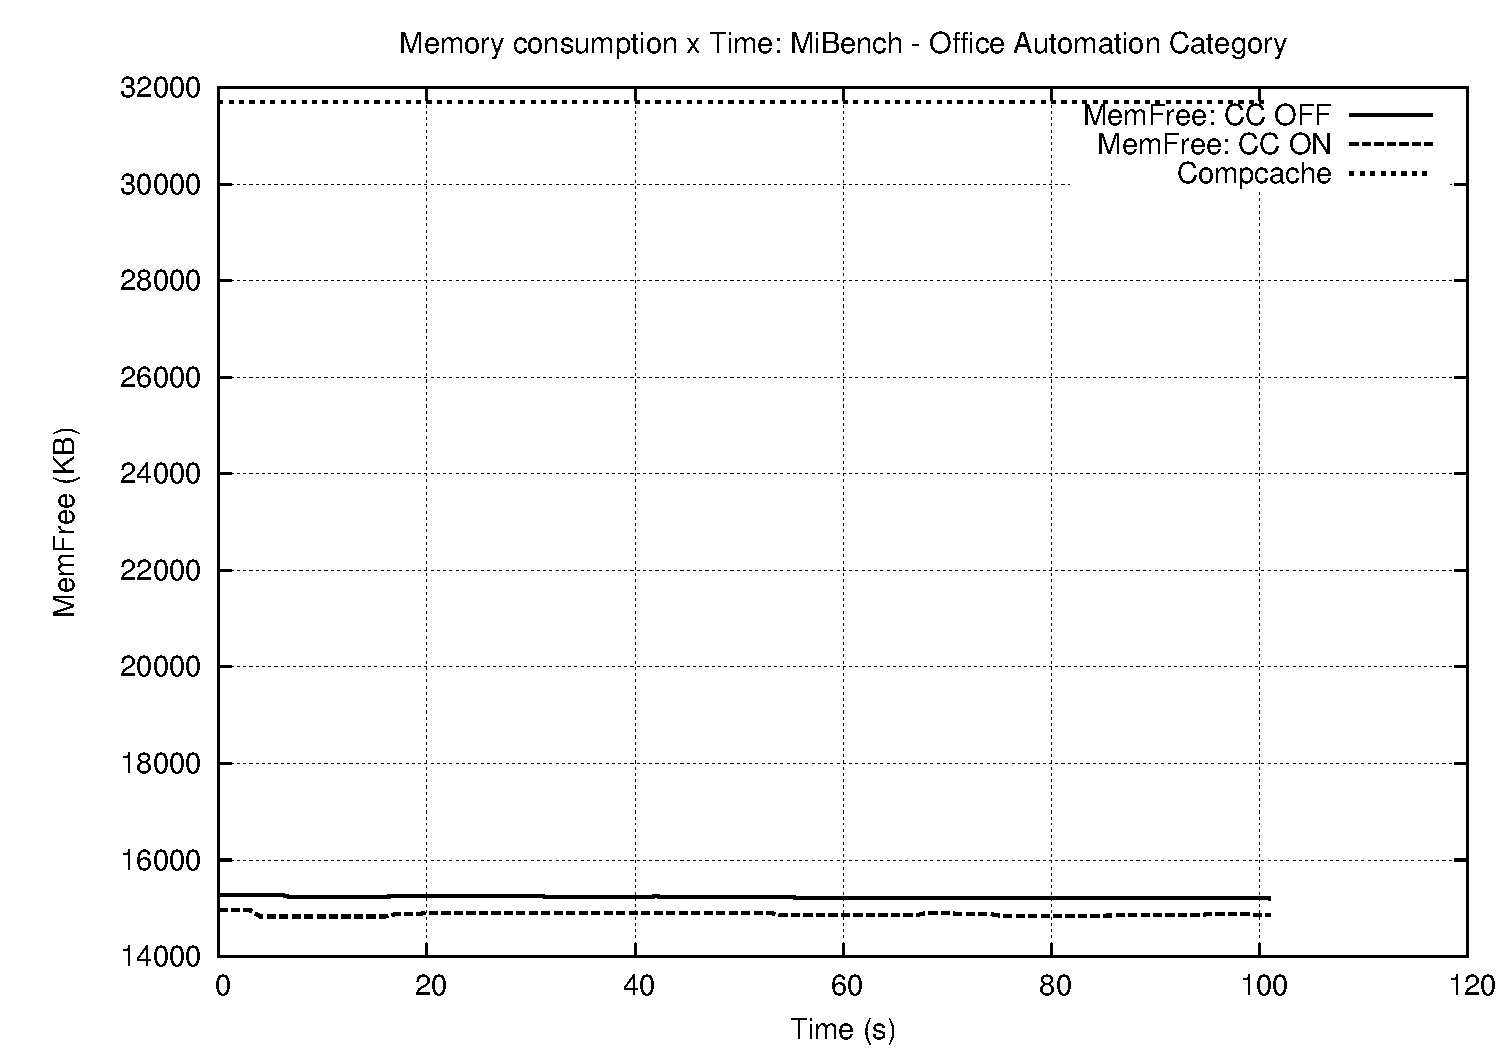
\includegraphics[scale=0.32]{figs/sbac-office}
 \caption{Compcache usage: Office Automation benchmarking}
 \label{fig:mibench_office}
\end{figure}

\begin{figure}[htpb]
 \centering
 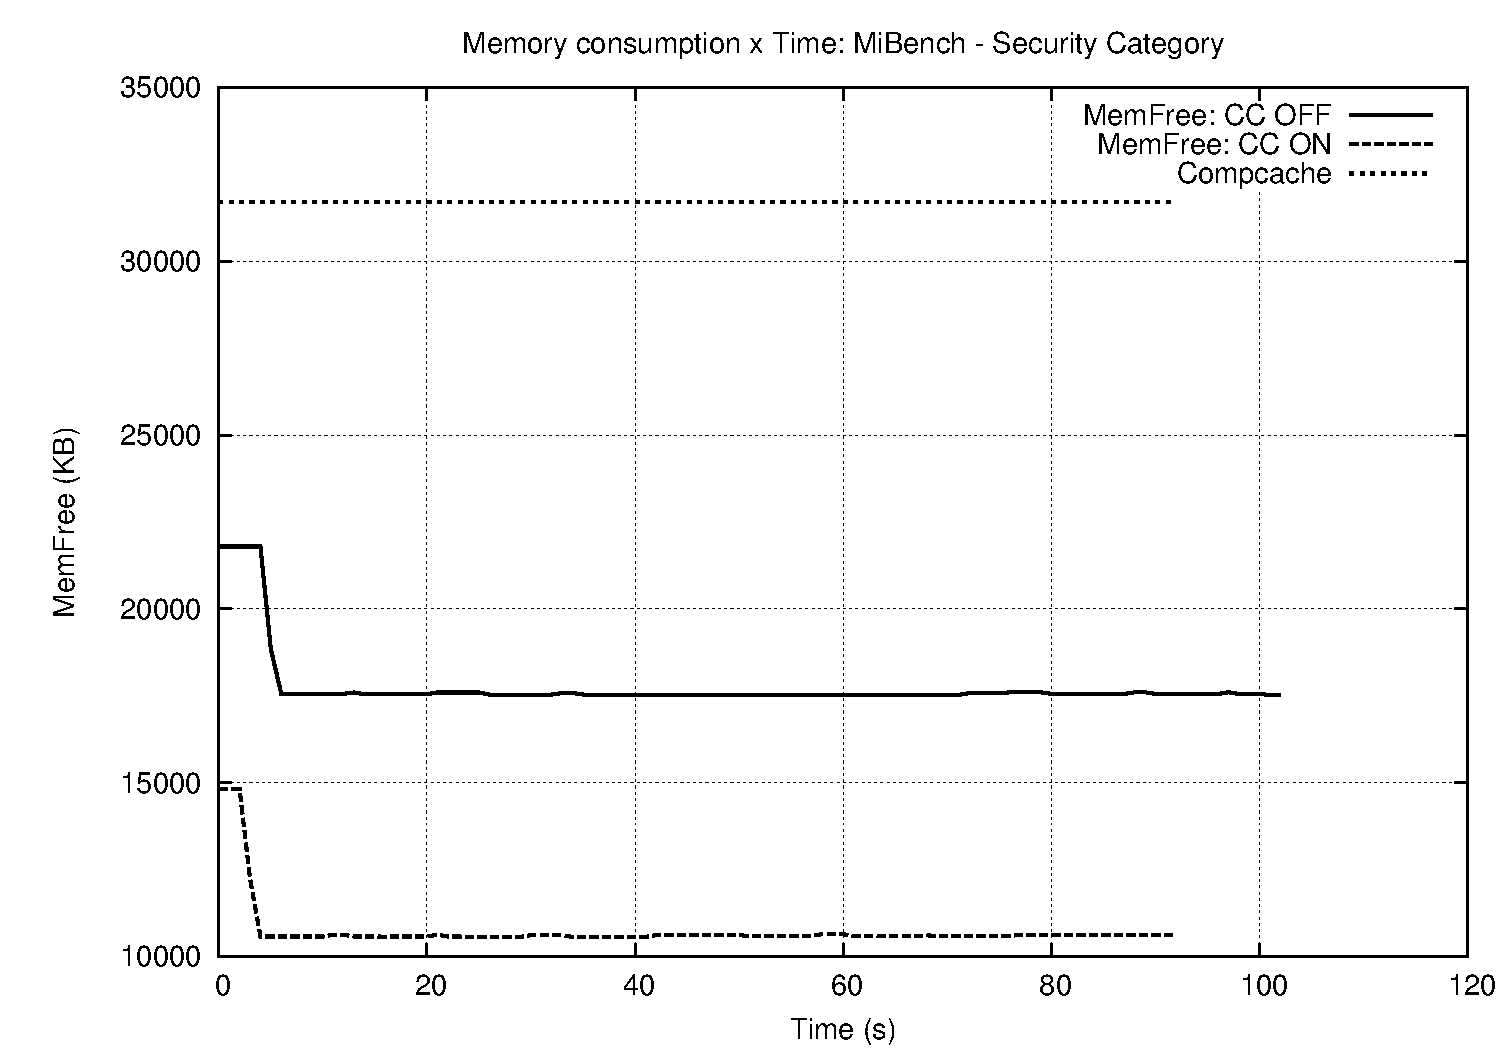
\includegraphics[scale=0.32]{figs/sbac-security}
 \caption{Compcache usage: Security benchmarking}
 \label{fig:mibench_security}
\end{figure}

\begin{figure}[htpb]
 \centering
 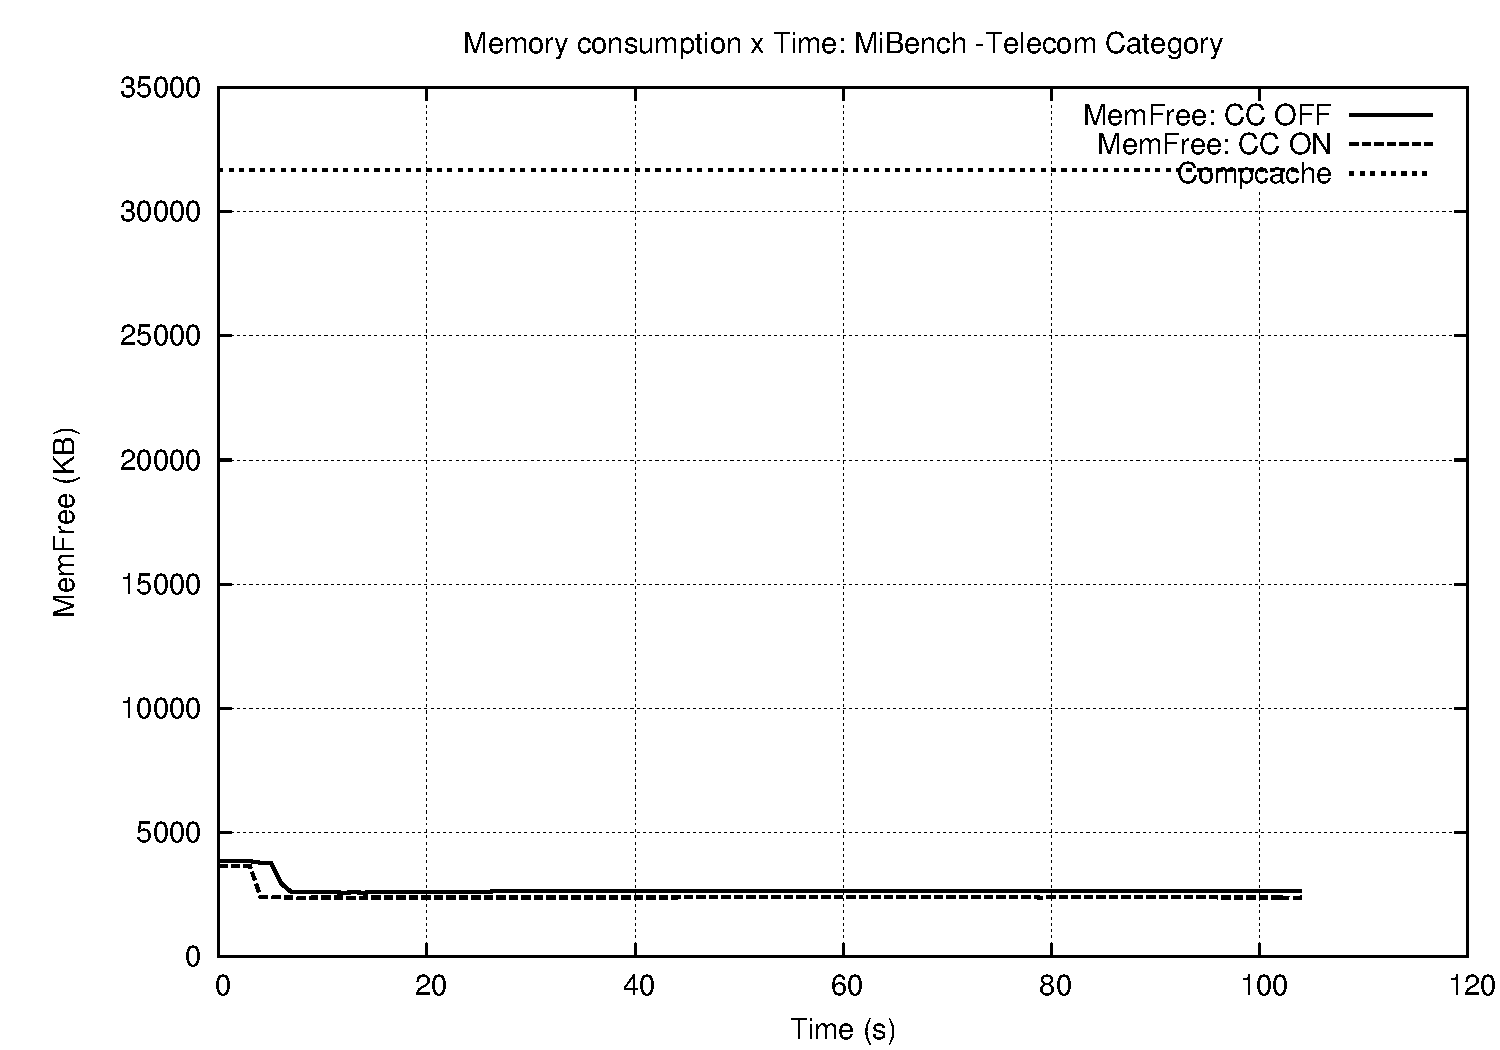
\includegraphics[scale=0.32]{figs/sbac-telecom}
 \caption{Compcache usage: Telecommunications benchmarking}
 \label{fig:mibench_telecom}
\end{figure}

Graphs presented in Figures \ref{fig:mibench_automotive}, \ref{fig:mibench_consumer}, \ref{fig:mibench_network}, \ref{fig:mibench_office}, \ref{fig:mibench_security}, \ref{fig:mibench_telecom}, Compcache utilization when MiBench benchmarks are executed did not bring any benefit to system performance or memory consumption. It happened due to low memory consumption by MiBench programs. Compcache is more effective when used in high memory consumption, compressing pages and keeping them in memory.
The gap between free memory available when Compcache is on have an explanation. Since ramzswap (the virtual memory area), takes a portion of free memory to allocate compressed pages, free memory is smaller when Compcache is added to system.

All graphs indicate that MiBench benchmarks are not ideal to evaluate memory consumption or Compcache performance. Was noted that MiBench benchmarks are designed to do more processor operations than memory operations. Due this, MiBench benchmarking could not evaluate Compcache performance.
}

\section{Related work}
\nohyphens{
The first implementation of compressed cache was done by Douglis \cite{douglis93} in 1993 and results were not conclusive. He achieved speed up for some applications, and slowdowns for others. Later, in 1999 Kaplan \cite{kaplan99compressed} pointed out that the machine Douglis used had a difference between the processor speed and the access times on hard disk that was much smaller than encountered nowadays. Kaplan also proposed a new adaptive scheme, since that used by Douglis was not conclusive about the applications' performance.

Following the same scheme, Rodrigo Castro \cite{castro03} implemented and evaluated compressed cache and compressed swap using the 2.4.x Linux kernel. He proposed a new approach to reduce fragmentation of the compressed pages, based on contiguous memory allocated areas---cells. He also proposed a new adaptability policy that adjusts the compressed cache size on the fly. Rodrigo's adaptive compressed cache approach is based on a tight compressed cache, without allocation of superfluous memory. The cells used by compressed cache are released to the system as soon as they are no longer needed. The compressed cache starts with a minimum size and as soon
as the VM system starts to evict pages, the compressed cache increases its memory usage in order to store them.

All those implementations are focused on desktop or server platforms. One implementation which is focused on embedded devices is CRAMES \cite{crames05}---Compressed RAM for embedded systems. CRAMES was implemented as a loadable module for the Linux kernel and evaluated on a battery-powered embedded system. CRAMES supports in-RAM compressed filesystems of any type and uses a chunks approach to store compressed pages and modifies the Operating System kernel to implement this approach.

The compressed cache implementation evaluated in this paper still does not have the adaptive feature implemented. From previous work, Compcache uses the same compression algorithms used by Rodrigo's implementation, but the storage of compressed pages is quite different. The implementation of dedicated memory allocator and the virtual swap approach reduces the fragmentation close to zero and speeds up the page recovery. Still, one of the major benefit is that Operating System kernel does not have to be changed.

Since Compcache evaluated in this paper is still under development, Open Source community and developers did not have tests in real embedded operating system. This paper is the first work done using latest Compcache version using real hardware and user applications.
}

\section{Conclusion}
\nohyphens{
Storing memory pages as compressed data decreases the number of access attempts to storage devices such as, for example, hard disks, which typically are accessed much slower than the main memory of a system. As such, we can observe more benefits when the difference between the access time to the main memory and the storage device is considerable. This characteristic is not typical for embedded Linux systems, and the benefits of storing pages as compressed data are much smaller than on an x86 architecture. Storage devices in the embedded Linux systems are typically flash memory, for instance MMC cards, and as we know, access times for these devices are much faster than access times for a hard disk. It allows us to come to the conclusion that wide use of Compcache is not justified in the embedded systems.

On the other hand, Compcache shows that is possible to avoid OOM call, improving the free memory available for user applications. Regarding the experiments, MiBench test suite presented that it is not designed for this kind of benchmarking. Since memory I/O is the focus for Compcache, MiBench did not able to measure the memory behavior or Compcache acting.
}
% All manuscripts must be in English.
% 
% %------------------------------------------------------------------------- 
% \SubSection{Printing your paper}
% 
% Print your properly formatted text on high-quality, $8.5 \times 11$-inch 
% white printer paper. A4 paper is also acceptable, but please leave the 
% extra 0.5 inch (1.27 cm) at the BOTTOM of the page.
% 
% %------------------------------------------------------------------------- 
% \SubSection{Margins and page numbering}
% 
% All printed material, including text, illustrations, and charts, must be 
% kept within a print area 6-7/8 inches (17.5 cm) wide by 8-7/8 inches 
% (22.54 cm) high. Do not write or print anything outside the print area. 
% Number your pages lightly, in pencil, on the upper right-hand corners of 
% the BACKS of the pages (for example, 1/10, 2/10, or 1 of 10, 2 of 10, and 
% so forth). Please do not write on the fronts of the pages, nor on the 
% lower halves of the backs of the pages.
% 
% 
% %------------------------------------------------------------------------ 
% \SubSection{Formatting your paper}
% 
% All text must be in a two-column format. The total allowable width of 
% the text area is 6-7/8 inches (17.5 cm) wide by 8-7/8 inches (22.54 cm) 
% high. Columns are to be 3-1/4 inches (8.25 cm) wide, with a 5/16 inch 
% (0.8 cm) space between them. The main title (on the first page) should 
% begin 1.0 inch (2.54 cm) from the top edge of the page. The second and 
% following pages should begin 1.0 inch (2.54 cm) from the top edge. On 
% all pages, the bottom margin should be 1-1/8 inches (2.86 cm) from the 
% bottom edge of the page for $8.5 \times 11$-inch paper; for A4 paper, 
% approximately 1-5/8 inches (4.13 cm) from the bottom edge of the page.
% 
% %------------------------------------------------------------------------- 
% \SubSection{Type-style and fonts}
% 
% Wherever Times is specified, Times Roman may also be used. If neither is 
% available on your word processor, please use the font closest in 
% appearance to Times that you have access to.
% 
% MAIN TITLE. Center the title 1-3/8 inches (3.49 cm) from the top edge of 
% the first page. The title should be in Times 14-point, boldface type. 
% Capitalize the first letter of nouns, pronouns, verbs, adjectives, and 
% adverbs; do not capitalize articles, coordinate conjunctions, or 
% prepositions (unless the title begins with such a word). Leave two blank 
% lines after the title.
% 
% AUTHOR NAME(s) and AFFILIATION(s) are to be centered beneath the title 
% and printed in Times 12-point, non-boldface type. This information is to 
% be followed by two blank lines.
% 
% The ABSTRACT and MAIN TEXT are to be in a two-column format. 
% 
% MAIN TEXT. Type main text in 10-point Times, single-spaced. Do NOT use 
% double-spacing. All paragraphs should be indented 1 pica (approx. 1/6 
% inch or 0.422 cm). Make sure your text is fully justified---that is, 
% flush left and flush right. Please do not place any additional blank 
% lines between paragraphs. Figure and table captions should be 10-point 
% Helvetica boldface type as in
% \begin{figure}[h]
%    \caption{Example of caption.}
% \end{figure}
% 
% \noindent Long captions should be set as in 
% \begin{figure}[h] 
%    \caption{Example of long caption requiring more than one line. It is 
%      not typed centered but aligned on both sides and indented with an 
%      additional margin on both sides of 1~pica.}
% \end{figure}
% 
% \noindent Callouts should be 9-point Helvetica, non-boldface type. 
% Initially capitalize only the first word of section titles and first-, 
% second-, and third-order headings.
% 
% FIRST-ORDER HEADINGS. (For example, {\large \bf 1. Introduction}) 
% should be Times 12-point boldface, initially capitalized, flush left, 
% with one blank line before, and one blank line after.
% 
% SECOND-ORDER HEADINGS. (For example, {\elvbf 1.1. Database elements}) 
% should be Times 11-point boldface, initially capitalized, flush left, 
% with one blank line before, and one after. If you require a third-order 
% heading (we discourage it), use 10-point Times, boldface, initially 
% capitalized, flush left, preceded by one blank line, followed by a period 
% and your text on the same line.
% 
% %------------------------------------------------------------------------- 
% \SubSection{Footnotes}
% 
% Please use footnotes sparingly%
% \footnote
%    {%
%      Or, better still, try to avoid footnotes altogether.  To help your 
%      readers, avoid using footnotes altogether and include necessary 
%      peripheral observations in the text (within parentheses, if you 
%      prefer, as in this sentence).
%    }
% and place them at the bottom of the column on the page on which they are 
% referenced. Use Times 8-point type, single-spaced.
% 
% 
% %------------------------------------------------------------------------- 
% \SubSection{References}
% 
% List and number all bibliographical references in 9-point Times, 
% single-spaced, at the end of your paper. When referenced in the text, 
% enclose the citation number in square brackets, for example~\cite{ex1}. 
% Where appropriate, include the name(s) of editors of referenced books.
% 
% %------------------------------------------------------------------------- 
% \SubSection{Illustrations, graphs, and photographs}
% 
% All graphics should be centered. Your artwork must be in place in the 
% article (preferably printed as part of the text rather than pasted up). 
% If you are using photographs and are able to have halftones made at a 
% print shop, use a 100- or 110-line screen. If you must use plain photos, 
% they must be pasted onto your manuscript. Use rubber cement to affix the 
% images in place. Black and white, clear, glossy-finish photos are 
% preferable to color. Supply the best quality photographs and 
% illustrations possible. Penciled lines and very fine lines do not 
% reproduce well. Remember, the quality of the book cannot be better than 
% the originals provided. Do NOT use tape on your pages!
% 
% %------------------------------------------------------------------------- 
% \SubSection{Color}
% 
% The use of color on interior pages (that is, pages other
% than the cover) is prohibitively expensive. We publish interior pages in 
% color only when it is specifically requested and budgeted for by the 
% conference organizers. DO NOT SUBMIT COLOR IMAGES IN YOUR 
% PAPERS UNLESS SPECIFICALLY INSTRUCTED TO DO SO.
% 
% %------------------------------------------------------------------------- 
% \SubSection{Symbols}
% 
% If your word processor or typewriter cannot produce Greek letters, 
% mathematical symbols, or other graphical elements, please use 
% pressure-sensitive (self-adhesive) rub-on symbols or letters (available 
% in most stationery stores, art stores, or graphics shops).
% 
% %------------------------------------------------------------------------ 
% \SubSection{Copyright forms}
% 
% You must include your signed IEEE copyright release form when you submit 
% your finished paper. We MUST have this form before your paper can be 
% published in the proceedings.
% 
% %------------------------------------------------------------------------- 
% \SubSection{Conclusions}
% 
% Please direct any questions to the production editor in charge of these 
% proceedings at the IEEE Computer Society Press: Phone (714) 821-8380, or 
% Fax (714) 761-1784.

%------------------------------------------------------------------------- 
%\nocite{ex1,ex2}
%\bibliographystyle{latex8}
%\bibliography{latex8}
\addcontentsline{toc}{section}{References}
\begin{flushleft}
	\bibliography{briglia-ref}
	\bibliographystyle{latex8}
\end{flushleft}

\end{document}

